\documentclass[conference]{IEEEtran}
\IEEEoverridecommandlockouts
% The preceding line is only needed to identify funding in the first footnote. If that is unneeded, please comment it out.
 
\usepackage{amsmath,amssymb,amsfonts}
\usepackage{algorithmic}
\usepackage{graphicx} 
\usepackage{textcomp}
\usepackage{xcolor} 
\usepackage[backend=biber]{biblatex}
\addbibresource{main.bib}

 \def\BibTeX{{\rm B\kern-.05em{\sc i\kern-.025em b}\kern-.08em
     T\kern-.1667em\lower.7ex\hbox{E}\kern-.125emX}}
    
\begin{document}
 
  
\title{Earth at night*\\
{\footnotesize \textsuperscript{*}The visualisation of average radiance in specific area}
}
 
\author{\IEEEauthorblockN{1\textsuperscript{st} Zhen Chen}
\IEEEauthorblockA{\textit{Faculty of Computing and Mathematical Sciences} \\
\textit{The University of Waikato}\\
Beijing, China \\
1561010}
\and
\IEEEauthorblockN{2\textsuperscript{nd} Huajie Xu}
\IEEEauthorblockA{\textit{dept. name of organization (of Aff.)} \\
\textit{name of organization (of Aff.)}\\
City, Country \\
email address or ORCID}
\and
\IEEEauthorblockN{3\textsuperscript{rd} Shengzhu Wang}
\IEEEauthorblockA{\textit{dept. name of organization (of Aff.)} \\
\textit{name of organization (of Aff.)}\\
City, Country \\
email address or ORCID}
\and
\IEEEauthorblockN{4\textsuperscript{th} Wenjie Tong}
\IEEEauthorblockA{\textit{dept. name of organization (of Aff.)} \\
\textit{name of organization (of Aff.)}\\
City, Country \\
email address or ORCID}
\and
\IEEEauthorblockN{5\textsuperscript{th} SiXiang Xiong}
\IEEEauthorblockA{\textit{dept. name of organization (of Aff.)} \\
\textit{name of organization (of Aff.)}\\
City, Country \\
email address or ORCID}
}

\maketitle

\begin{abstract}
This document is the description about the solution of Assignment 2 of Compx527 paper in Waikato University. World Bank Nightime Light Data consists of a lot of satellite imagery stored in Amazon Web Services (AWS). Recent files from 2012-2020 are generated by the sensors named Visible Infrared Imaging Radiometer Suite Day-Night Band (VIIRS DNB). All the things are stored by Cloud Optimized GeoTIFF (COG) format and organized by Spatial Temporal Asset Catalog (STAC) standard. This project only researches the imagery from 3 specific areas. From them, you can learn the trend of their radiance in the period. It is also a good chance to have a better understanding of ecnomic trend by them. 
\end{abstract}

\begin{IEEEkeywords}
Night light, STAC, COG, VIIRS DNB, AWS
\end{IEEEkeywords}

\section{Solution Summary}
A lot of services are depended by this project. It is important to know that imagery from AWS open datasets has almost not processed too much before storing. So the Geospatial Data Abstraction Library (GDAL) is imported for the complicated computing. In addition, to ensure our project development schedule, Lark, which is a kind of instant messenger used in Chinese office, is used to record documents and communicate in a group. The architecture of our solution is shown as below.

\begin{figure}[htbp]
    \centerline{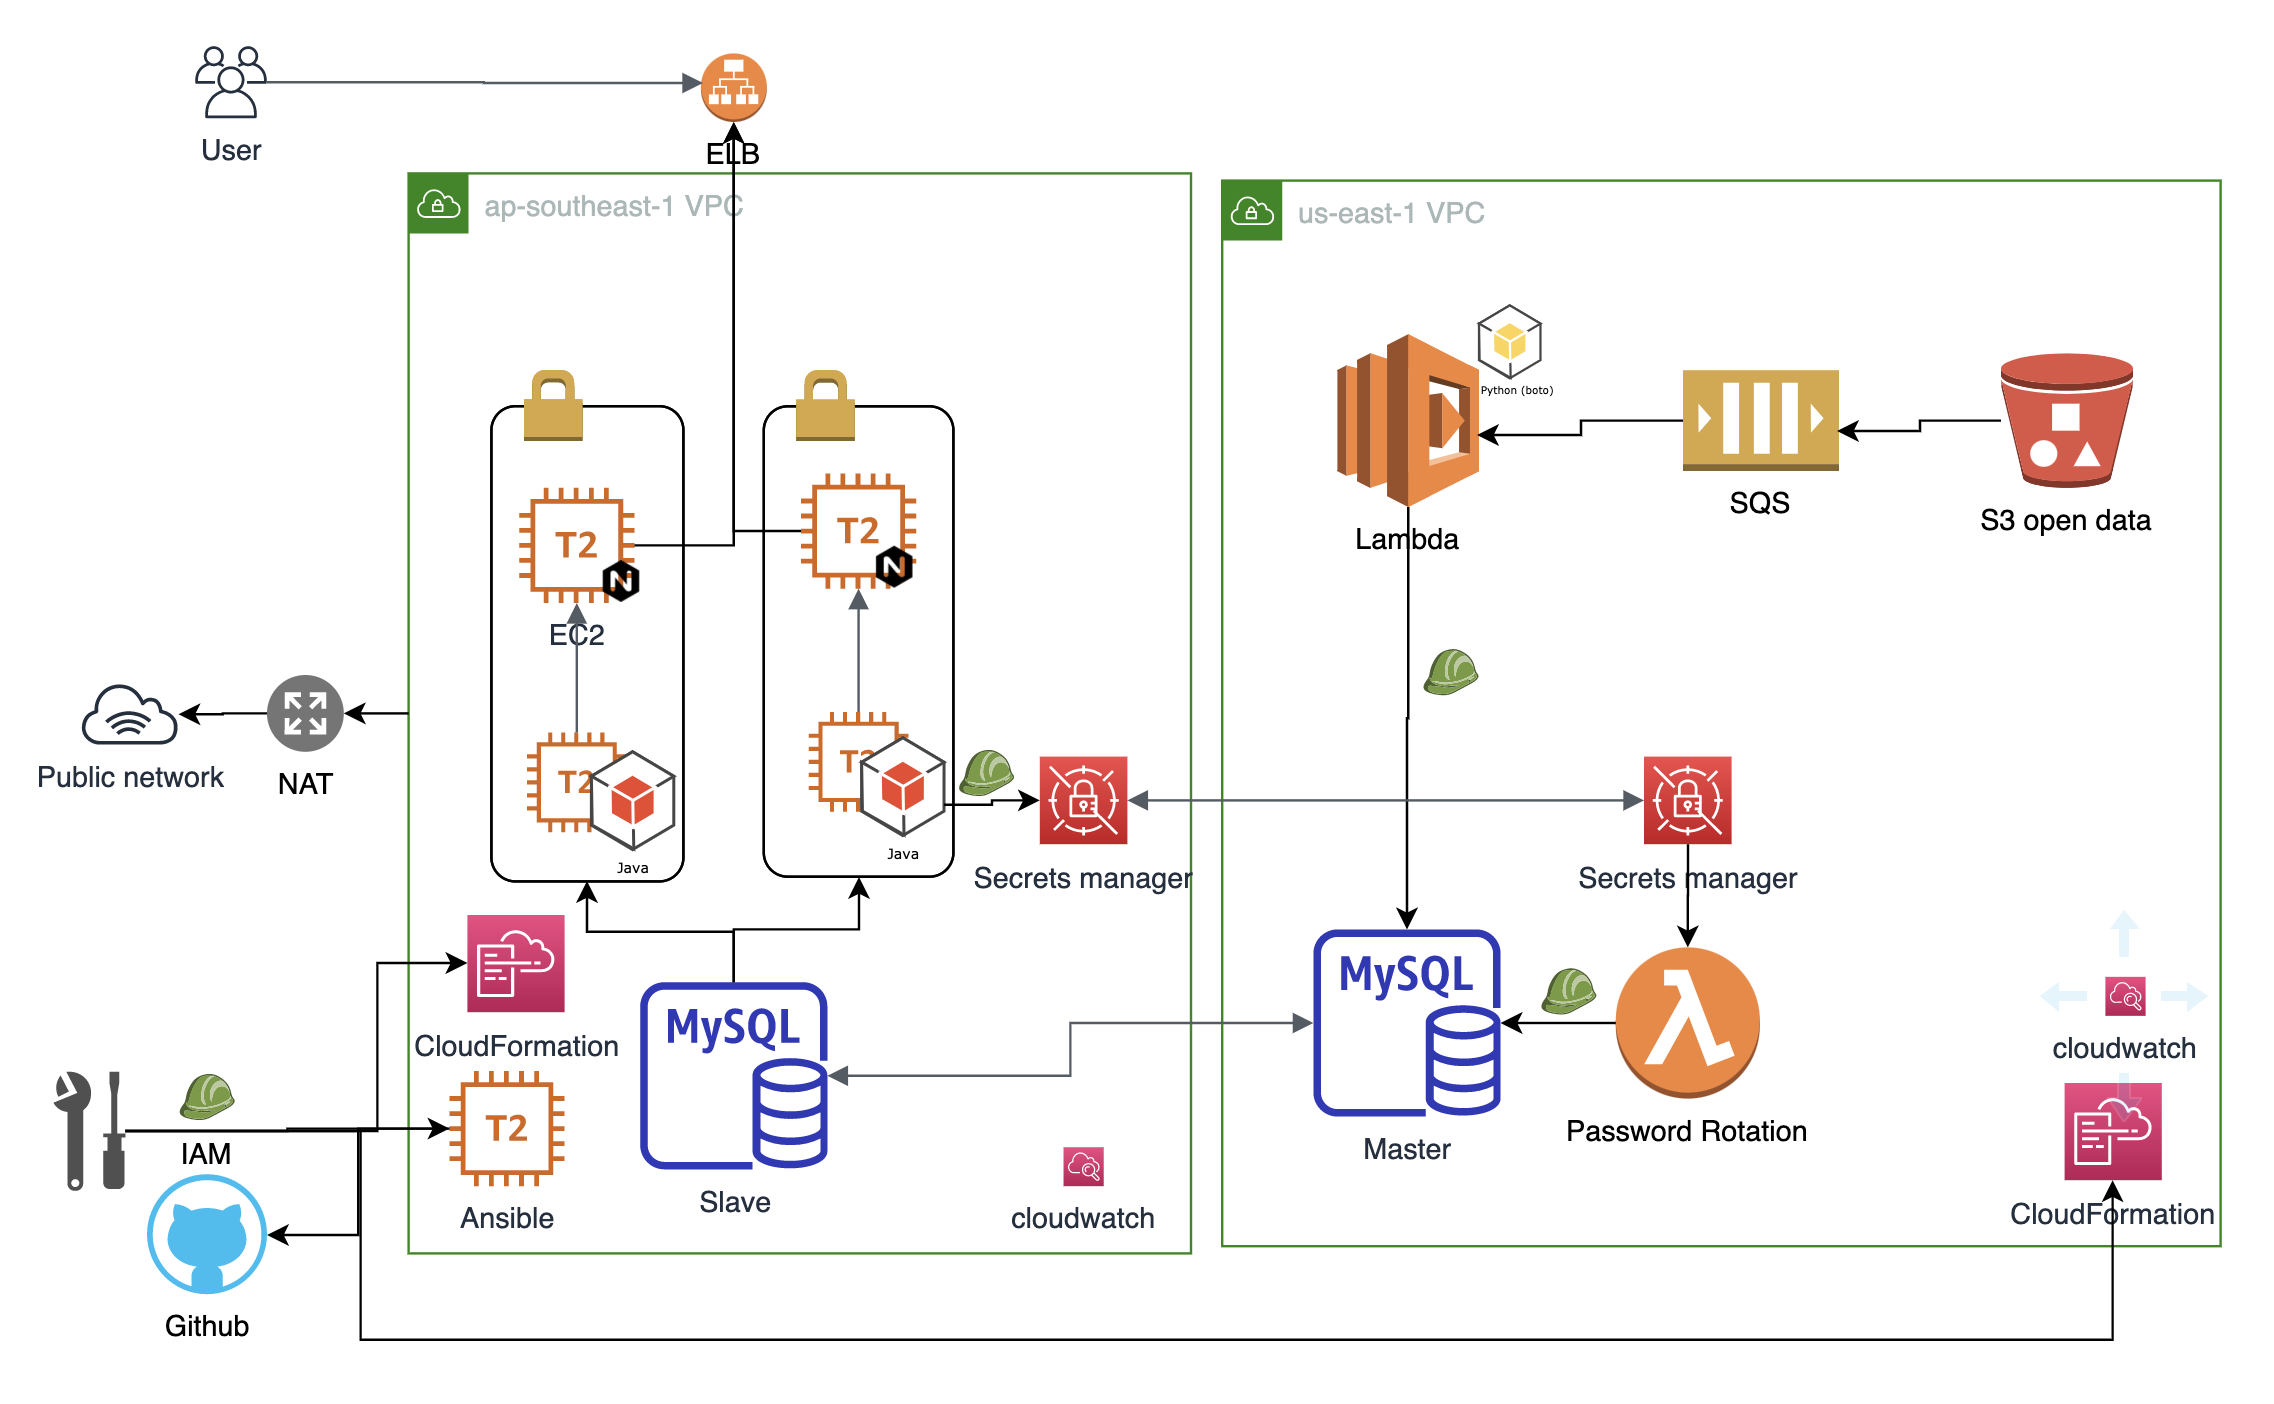
\includegraphics[width=260pt]{images/arch.png}}
    \caption{Architecture}
    \label{fig1}
\end{figure}
    
Figure Labels: To process the S3 data, two Lambda functions are generated. One is to follow the STAC protcol to find the imagery, and another is to analyse the picture by GDAL, which is a kind of high cost computation. There are more than 4 pictures per day per area, and more than 5,000 pictures per month totally. All the result processed by Lambda is stored in RDS and synced from us-east-1 region to ap-southeast-1 region. In addition, the password of MySQL are generated by a Lambda function and rotated timely. So the development team do not need to copy the password. Any feature with the password have to get it from Secrets Manager.  

When it comes to show the result in ap-southeast-1 region, networking security is the most essential thing because this part of service can be touched by end users. So except ELB server and deployment server, there are not any other servers with public ip. All the EC2 can visit public network from the NAT, but public network can not visit them directly.


\subsection{Open Nighttime Lights}
this is the explaination  \cite{BARA2020106658}

\subsection{Frontend}
this is the explanation

\subsection{vue}
this is the explanation

\subsection{D3}
this is the explanation
 
\subsection{spring-boot}
this is the explanation

\subsection{oauth github}
this is the explanation

\subsection{ansible}
Ansible is a famous open source deployment platform. 

\subsection{CloudFormation}
CloudFormation is a service in AWS, which can organize our service very quickly and no codes need to write. The configuration in CloudFormation is a template which is just a yaml file. It is more convient than Ansible for some services. We use it deploy the RDS and Lambda Service.

\subsection{nginx/tomcat}
Nginx is the widely used web server all over the world. It also has the excellent performance as a reverse proxy. We use it as our fontend server. Tomcat is a tranditional Java web container supporting Java Servlet. Our Java code run on Tomcat. 

\subsection{RDS/Lambda/secrets manager/SQS/EC2}
These items are the name of services on AWS. Especially, we use Lambda to generate temperary password of RDS, and store it in Secrets Manager. It is a good method to enhance the security of database password.

\section{Proposed solution}

\subsection{Whole structure}
A architecture pic.

\subsection{Frontend}

\subsection{Login}

\subsection{Data processing}

\subsection{Testing}

\subsection{Project management}

\section{Security Considerations}

\subsection{Networking}

\subsection{User}

\subsection{IAM}

\section{Team members and individual contribution within the team}
\begin{itemize}
    \item Zhen Chen:  PM, BE, DevOps
    \item Huajie Xu: FE
    \item Shengzhu Wang(Simon): BE
    \item SiXiang Xiong(Tom): BE, Testing
    \item Wenjie Tong: Data Researcher, Testing
\end{itemize}

\subsection{Equations}
Number equations consecutively. To make your 
equations more compact, you may use the solidus (~/~), the exp function, or 
appropriate exponents. Italicize Roman symbols for quantities and variables, 
but not Greek symbols. Use a long dash rather than a hyphen for a minus 
sign. Punctuate equations with commas or periods when they are part of a 
sentence, as in:
\begin{equation}
a+b=\gamma\label{eq}
\end{equation}

Be sure that the 
symbols in your equation have been defined before or immediately following 
the equation. Use ``\eqref{eq}'', not ``Eq.~\eqref{eq}'' or ``equation \eqref{eq}'', except at 
the beginning of a sentence: ``Equation \eqref{eq} is . . .''

\subsection{\LaTeX-Specific Advice}

Please use ``soft'' (e.g., \verb|\eqref{Eq}|) cross references instead
of ``hard'' references (e.g., \verb|(1)|). That will make it possible
to combine sections, add equations, or change the order of figures or
citations without having to go through the file line by line.

Please don't use the \verb|{eqnarray}| equation environment. Use
\verb|{align}| or \verb|{IEEEeqnarray}| instead. The \verb|{eqnarray}|
environment leaves unsightly spaces around relation symbols.

Please note that the \verb|{subequations}| environment in {\LaTeX}
will increment the main equation counter even when there are no
equation numbers displayed. If you forget that, you might write an
article in which the equation numbers skip from (17) to (20), causing
the copy editors to wonder if you've discovered a new method of
counting.

{\BibTeX} does not work by magic. It doesn't get the bibliographic
data from thin air but from .bib files. If you use {\BibTeX} to produce a
bibliography you must send the .bib files. 

{\LaTeX} can't read your mind. If you assign the same label to a
subsubsection and a table, you might find that Table I has been cross
referenced as Table IV-B3. 

{\LaTeX} does not have precognitive abilities. If you put a
\verb|\label| command before the command that updates the counter it's
supposed to be using, the label will pick up the last counter to be
cross referenced instead. In particular, a \verb|\label| command
should not go before the caption of a figure or a table.

Do not use \verb|\nonumber| inside the \verb|{array}| environment. It
will not stop equation numbers inside \verb|{array}| (there won't be
any anyway) and it might stop a wanted equation number in the
surrounding equation.

\subsection{Some Common Mistakes}\label{SCM}
\begin{itemize}
\item The word ``data'' is plural, not singular.
\item The subscript for the permeability of vacuum $\mu_{0}$, and other common scientific constants, is zero with subscript formatting, not a lowercase letter ``o''.
\item In American English, commas, semicolons, periods, question and exclamation marks are located within quotation marks only when a complete thought or name is cited, such as a title or full quotation. When quotation marks are used, instead of a bold or italic typeface, to highlight a word or phrase, punctuation should appear outside of the quotation marks. A parenthetical phrase or statement at the end of a sentence is punctuated outside of the closing parenthesis (like this). (A parenthetical sentence is punctuated within the parentheses.)
\item A graph within a graph is an ``inset'', not an ``insert''. The word alternatively is preferred to the word ``alternately'' (unless you really mean something that alternates).
\item Do not use the word ``essentially'' to mean ``approximately'' or ``effectively''.
\item In your paper title, if the words ``that uses'' can accurately replace the word ``using'', capitalize the ``u''; if not, keep using lower-cased.
\item Be aware of the different meanings of the homophones ``affect'' and ``effect'', ``complement'' and ``compliment'', ``discreet'' and ``discrete'', ``principal'' and ``principle''.
\item Do not confuse ``imply'' and ``infer''.
\item The prefix ``non'' is not a word; it should be joined to the word it modifies, usually without a hyphen.
\item There is no period after the ``et'' in the Latin abbreviation ``et al.''.
\item The abbreviation ``i.e.'' means ``that is'', and the abbreviation ``e.g.'' means ``for example''.
\end{itemize}

\subsection{Authors and Affiliations}
\textbf{The class file is designed for, but not limited to, six authors.} A 
minimum of one author is required for all conference articles. Author names 
should be listed starting from left to right and then moving down to the 
next line. This is the author sequence that will be used in future citations 
and by indexing services. Names should not be listed in columns nor group by 
affiliation. Please keep your affiliations as succinct as possible (for 
example, do not differentiate among departments of the same organization).

\subsection{Identify the Headings}
Headings, or heads, are organizational devices that guide the reader through 
your paper. There are two types: component heads and text heads.

Component heads identify the different components of your paper and are not 
topically subordinate to each other. Examples include Acknowledgments and 
References and, for these, the correct style to use is ``Heading 5''. Use 
``figure caption'' for your Figure captions, and ``table head'' for your 
table title. Run-in heads, such as ``Abstract'', will require you to apply a 
style (in this case, italic) in addition to the style provided by the drop 
down menu to differentiate the head from the text.

Text heads organize the topics on a relational, hierarchical basis. For 
example, the paper title is the primary text head because all subsequent 
material relates and elaborates on this one topic. If there are two or more 
sub-topics, the next level head (uppercase Roman numerals) should be used 
and, conversely, if there are not at least two sub-topics, then no subheads 
should be introduced.

\subsection{Figures and Tables}
\paragraph{Positioning Figures and Tables} Place figures and tables at the top and 
bottom of columns. Avoid placing them in the middle of columns. Large 
figures and tables may span across both columns. Figure captions should be 
below the figures; table heads should appear above the tables. Insert 
figures and tables after they are cited in the text. Use the abbreviation 
``Fig.~\ref{fig}'', even at the beginning of a sentence.

\begin{table}[htbp]
\caption{Table Type Styles}
\begin{center}
\begin{tabular}{|c|c|c|c|}
\hline
\textbf{Table}&\multicolumn{3}{|c|}{\textbf{Table Column Head}} \\
\cline{2-4} 
\textbf{Head} & \textbf{\textit{Table column subhead}}& \textbf{\textit{Subhead}}& \textbf{\textit{Subhead}} \\
\hline
copy& More table copy$^{\mathrm{a}}$& &  \\
\hline
\multicolumn{4}{l}{$^{\mathrm{a}}$Sample of a Table footnote.}
\end{tabular}
\label{tab1}
\end{center}
\end{table}

\begin{figure}[htbp]
\centerline{
\includegraphics{fig1.png}}
\caption{Example of a figure caption.}
\label{fig}
\end{figure}

Figure Labels: Use 8 point Times New Roman for Figure labels. Use words 
rather than symbols or abbreviations when writing Figure axis labels to 
avoid confusing the reader. As an example, write the quantity 
``Magnetization'', or ``Magnetization, M'', not just ``M''. If including 
units in the label, present them within parentheses. Do not label axes only 
with units. In the example, write ``Magnetization (A/m)'' or ``Magnetization 
\{A[m(1)]\}'', not just ``A/m''. Do not label axes with a ratio of 
quantities and units. For example, write ``Temperature (K)'', not 
``Temperature/K''.

\section*{Acknowledgment}

The preferred spelling of the word ``acknowledgment'' in America is without 
an ``e'' after the ``g''. Avoid the stilted expression ``one of us (R. B. 
G.) thanks $\ldots$''. Instead, try ``R. B. G. thanks$\ldots$''. Put sponsor 
acknowledgments in the unnumbered footnote on the first page.

\section*{References}
 

Number footnotes separately in superscripts. Place the actual footnote at 
the bottom of the column in which it was cited. Do not put footnotes in the 
abstract or reference list. Use letters for table footnotes.

Unless there are six authors or more give all authors' names; do not use 
``et al.''. Papers that have not been published, even if they have been  

\printbibliography
 
\vspace{12pt}
\color{red}
IEEE conference templates contain guidance text for composing and formatting conference papers. Please ensure that all template text is removed from your conference paper prior to submission to the conference. Failure to remove the template text from your paper may result in your paper not being published.

\end{document}
